% Source PDF page 325 (printed p. 311)
\begin{figure}[htbp]\centering
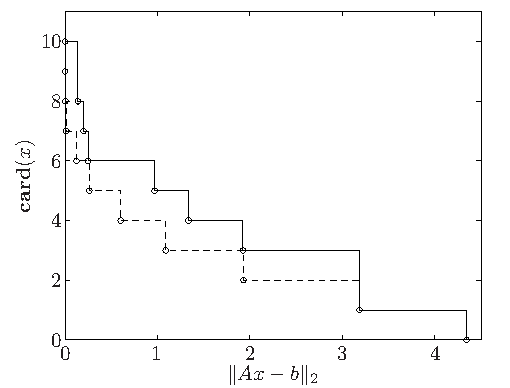
\includegraphics[width=.65\textwidth]{ch06-07.pdf}
\caption*{图6.7\quad 对矩阵 $A\in\R^{10\times20}$ 进行稀疏回归向量选择。虚线上的圆圈，是残差 $\norm{Ax-b}_2$ 与非零元素数 $\operatorname{card}(x)$ 之间权衡的 Pareto 最优值。实线上以圆圈标出的点，由 $\ell_1$ 范数正则化启发式方法得到。}
\end{figure}
信号 $x$ 被加性噪声 $v$ 污染：
\[x_{\rm cor}=x+v.\]
噪声可以用许多不同方式建模，这里只假定它未知、较小，并且与信号不同，它变化迅速。目标是给定受污染信号 $x_{\rm cor}$，构造原信号 $x$ 的估计 $\widehat x$。这个过程称为\emph{信号重构}，因为要从受污染的版本中重构原信号；也称为\emph{去噪}，因为要从受污染的信号中除去噪声。大多数重构方法最终都会对 $x_{\rm cor}$ 作某种平滑操作而得到 $\widehat x$，因此这个过程也称为\emph{平滑}。

重构问题的一种简单表述是双准则问题
\begin{equation}
\text{相对于 }\R_+^2\text{ 最小化}\quad(\norm{\widehat x-x_{\rm cor}}_2,\phi(\widehat x)),\tag{6.12}
\end{equation}
其中 $\widehat x$ 是变量，$x_{\rm cor}$ 是问题参数。函数 $\phi:\R^n\to\R$ 是凸函数，称为\emph{正则化函数}或\emph{平滑目标}，用于衡量估计 $\widehat x$ 的粗糙程度或不平滑程度。重构问题 (6.12) 寻找与受污染信号接近（按 $\ell_2$ 范数衡量）、同时又平滑（$\phi(\widehat x)$ 较小）的信号。问题 (6.12) 是凸双准则问题，可以通过标量化并求解一个标量凸优化问题，得到 Pareto 最优点。

% Source PDF page 326 (printed p. 312)
\subsubsection*{二次平滑}
最简单的重构方法采用二次平滑函数
\[\phi_{\rm quad}(x)=\sum_{i=1}^{n-1}(x_{i+1}-x_i)^2=\norm{Dx}_2^2,\]
其中 $D\in\R^{(n-1)\times n}$ 是双对角矩阵
\[D=\begin{bmatrix}-1&1&0&\cdots&0&0&0\\0&-1&1&\cdots&0&0&0\\\vdots&\vdots&\vdots&&\vdots&\vdots&\vdots\\0&0&0&\cdots&-1&1&0\\0&0&0&\cdots&0&-1&1\end{bmatrix}.\]
通过最小化
\[\norm{\widehat x-x_{\rm cor}}_2^2+\delta\norm{D\widehat x}_2^2,\]
可以得到 $\norm{\widehat x-x_{\rm cor}}_2$ 与 $\norm{D\widehat x}_2$ 的最优权衡，其中 $\delta>0$ 将最优权衡曲线参数化。该二次问题的解为
\[\widehat x=(I+\delta D^\T D)^{-1}x_{\rm cor}.\]
由于 $I+\delta D^\T D$ 是三对角矩阵，这个解可以非常高效地计算，见附录C。

\subsubsection*{二次平滑的例子}
图6.8给出信号 $x\in\R^{4000}$（上）及受污染信号 $x_{\rm cor}$（下）。目标 $\norm{\widehat x-x_{\rm cor}}_2$ 与 $\norm{D\widehat x}_2$ 的最优权衡曲线见图6.9。曲线最左端对应 $\widehat x=x_{\rm cor}$，目标值为 $\norm{Dx_{\rm cor}}_2=4.4$；最右端对应 $\widehat x=0$，此时 $\norm{\widehat x-x_{\rm cor}}_2=\norm{x_{\rm cor}}_2=16.2$。注意，曲线在 $\norm{\widehat x-x_{\rm cor}}_2\approx3$ 附近有明显拐弯。

图6.10给出最优权衡曲线上的三个平滑信号，分别对应 $\norm{\widehat x-x_{\rm cor}}_2=8$（上）、$3$（中）和 $1$（下）。把重构信号与原信号 $x$ 比较，可见 $\norm{\widehat x-x_{\rm cor}}_2=3$ 时的重构最好，正对应权衡曲线的拐弯处。$\norm{\widehat x-x_{\rm cor}}_2$ 更大时，平滑过度；更小时，平滑不足。

\subsubsection*{全变差重构}
当原信号十分平滑，而噪声变化迅速时，简单的二次平滑是一种很好的重构方法。但显然，原信号中的任何快速变化也都会被二次平滑削弱或消除。本节介绍一种既能消除大部分噪声，又能保留原信号中偶尔出现的快速变化的重构方法。该方法基于平滑函数
\[\phi_{\rm tv}(\widehat x)=\sum_{i=1}^{n-1}|\widehat x_{i+1}-\widehat x_i|=\norm{D\widehat x}_1,\]
它称为 $x\in\R^n$ 的\emph{全变差}。

% Source PDF page 327 (printed p. 313)
\begin{figure}[htbp]\centering
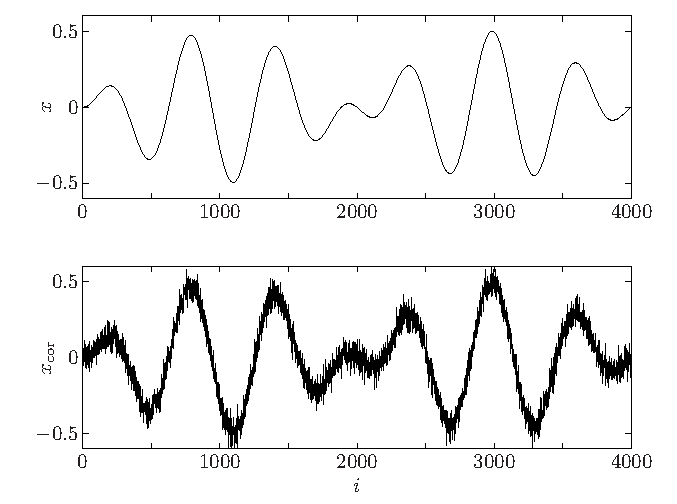
\includegraphics[width=.85\textwidth]{ch06-08.pdf}
\caption*{图6.8\quad 上：原信号 $x\in\R^{4000}$。下：受污染信号 $x_{\rm cor}$。}
\end{figure}
\begin{figure}[htbp]\centering
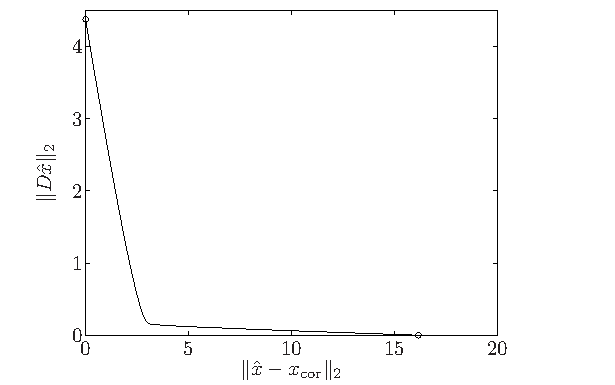
\includegraphics[width=.65\textwidth]{ch06-09.pdf}
\caption*{图6.9\quad $\norm{D\widehat x}_2$ 与 $\norm{\widehat x-x_{\rm cor}}_2$ 之间的最优权衡曲线。在 $\norm{\widehat x-x_{\rm cor}}\approx3$ 附近，曲线有明显拐弯。}
\end{figure}

% Source PDF page 328 (printed p. 314)
\begin{figure}[htbp]\centering
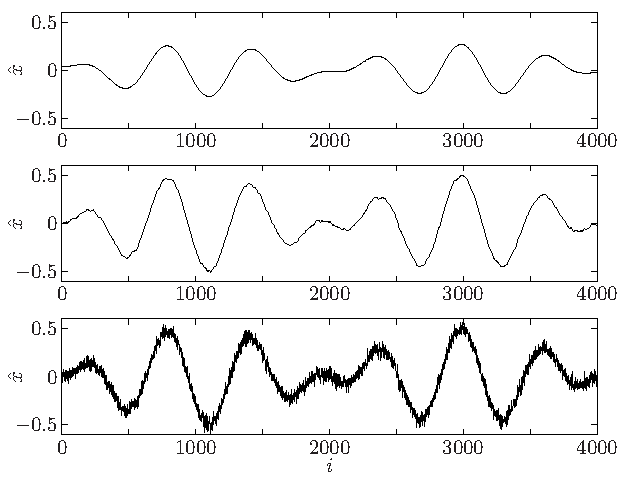
\includegraphics[width=.82\textwidth]{ch06-10.pdf}
\caption*{图6.10\quad 三个平滑或重构后的信号 $\widehat x$。上图对应 $\norm{\widehat x-x_{\rm cor}}_2=8$，中图对应 $\norm{\widehat x-x_{\rm cor}}_2=3$，下图对应 $\norm{\widehat x-x_{\rm cor}}_2=1$。}
\end{figure}
与二次平滑程度指标 $\phi_{\rm quad}$ 类似，全变差函数对变化迅速的 $\widehat x$ 赋予较大的值。不过，全变差指标对较大的 $|x_{i+1}-x_i|$ 赋予的惩罚相对较小。

\subsubsection*{全变差重构的例子}
图6.11给出信号 $x\in\R^{2000}$（上图）以及受噪声污染的信号 $x_{\rm cor}$。信号大体平滑，但有几处快速变化或跳变；噪声则变化迅速。

先采用二次平滑。图6.12给出 $\norm{D\widehat x}_2$ 与 $\norm{\widehat x-x_{\rm cor}}_2$ 最优权衡曲线上的三个平滑信号。在前两个信号中，原信号的快速变化也被平滑了。在第三个信号中，陡峭边缘保留得较好，但仍有大量噪声。

再来看全变差重构。图6.13是 $\norm{D\widehat x}_1$ 与 $\norm{\widehat x-x_{\rm cor}}_2$ 的最优权衡曲线。图6.14给出该曲线上对应 $\norm{D\widehat x}_1=5$（上）、$8$（中）和 $10$（下）的重构信号。可以看到，与二次平滑不同，全变差重构保留了信号中的突变。

% Source PDF page 329 (printed p. 315)
\begin{figure}[htbp]\centering
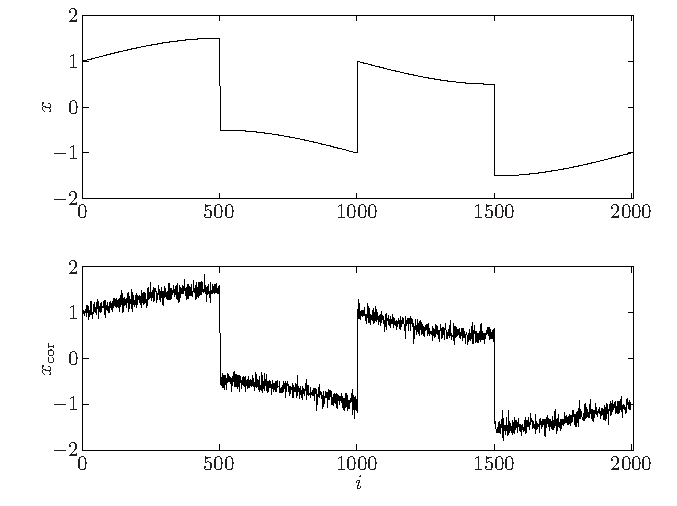
\includegraphics[width=.85\textwidth]{ch06-11.pdf}
\caption*{图6.11\quad 信号 $x\in\R^{2000}$ 及受污染信号 $x_{\rm cor}\in\R^{2000}$。噪声变化迅速，而信号大体平滑，只有几处快速变化。}
\end{figure}

% Source PDF page 330 (printed p. 316)
\begin{figure}[htbp]\centering
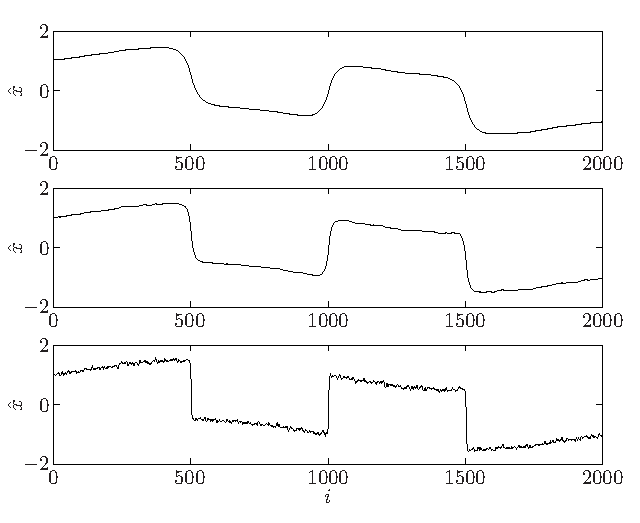
\includegraphics[width=.82\textwidth]{ch06-12.pdf}
\caption*{图6.12\quad 三个经二次平滑的信号 $\widehat x$。上图对应 $\norm{\widehat x-x_{\rm cor}}_2=10$，中图对应 $7$，下图对应 $4$。上图大幅降低噪声，但也过度平滑了信号中的快速变化。最下方的平滑信号降噪不足，同时仍平滑了原信号的快速变化。中间信号给出了最好的折中，但仍会平滑快速变化。}
\end{figure}
\begin{figure}[htbp]\centering
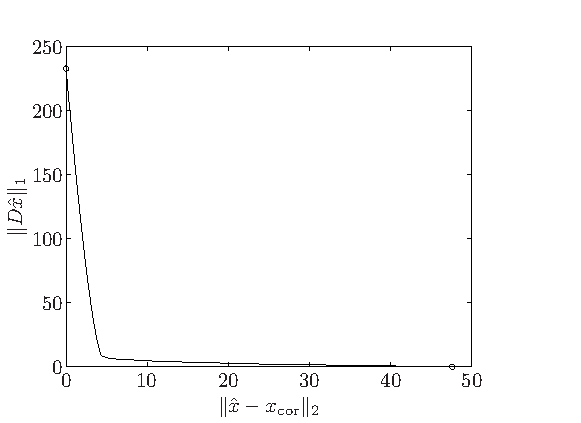
\includegraphics[width=.68\textwidth]{ch06-13.pdf}
\caption*{图6.13\quad $\norm{D\widehat x}_1$ 与 $\norm{\widehat x-x_{\rm cor}}_2$ 之间的最优权衡曲线。}
\end{figure}

% Source PDF page 331 (printed p. 317)
\begin{figure}[htbp]\centering
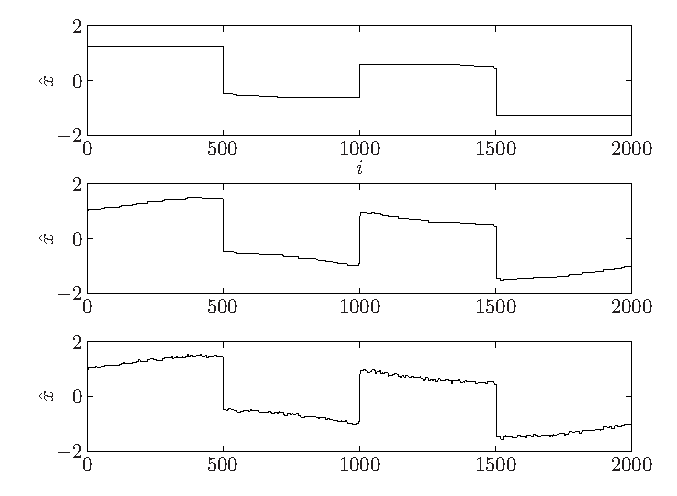
\includegraphics[width=.85\textwidth]{ch06-14.pdf}
\caption*{图6.14\quad 采用全变差重构得到的三个信号 $\widehat x$。上图对应 $\norm{D\widehat x}_1=5$，中图对应 $8$，下图对应 $10$。下图的噪声消除稍显不足，上图则消除了信号中一些缓慢变化的部分。注意，与二次平滑不同，全变差重构保留了信号中的突变。}
\end{figure}

% Source PDF page 332 (printed p. 318)
\section{稳健逼近}
\subsection{随机稳健逼近}
考虑基本目标为 $\norm{Ax-b}$ 的逼近问题，同时希望考虑数据矩阵 $A$ 的不确定性或可能变化。（同样的想法可以扩展到 $A$、$b$ 都不确定的情形。）本节用统计模型描述 $A$ 的变化。

假设 $A$ 是取值于 $\R^{m\times n}$、均值为 $\overline A$ 的随机变量，因此可以写为
\[A=\overline A+U,\]
其中 $U$ 是零均值随机矩阵。常矩阵 $\overline A$ 给出 $A$ 的平均值，$U$ 描述它的统计变化。

自然可以用 $\norm{Ax-b}$ 的期望作为目标：
\begin{equation}\text{最小化}\quad\E\norm{Ax-b}.\tag{6.13}\end{equation}
称其为\emph{随机稳健逼近问题}。它总是一个凸优化问题，但通常难以处理，因为在大多数情况下，计算目标或其导数都非常困难。

当 $A$ 只取有限个值时，随机稳健逼近问题 (6.13) 可以求解。这是一个简单情形，即
\[\Prob(A=A_i)=p_i,\qquad i=1,\ldots,k,\]
其中 $A_i\in\R^{m\times n}$、$\one^\T p=1$、$p\succeq0$。此时问题 (6.13) 为
\[\text{最小化}\quad p_1\norm{A_1x-b}+\cdots+p_k\norm{A_kx-b},\]
通常称为\emph{范数和问题}。它可表示为
\[\begin{array}{ll}\text{最小化}&p^\T t\\\text{约束条件}&\norm{A_ix-b}\le t_i,\quad i=1,\ldots,k,\end{array}\]
变量为 $x\in\R^n$、$t\in\R^k$。如果范数是欧几里得范数，这个范数和问题就是 SOCP。如果采用 $\ell_1$ 或 $\ell_\infty$ 范数，则可写为 LP，见习题6.8。

随机稳健逼近问题 (6.13) 的一些变体是可处理的。例如，考虑随机稳健最小二乘问题
\[\text{最小化}\quad\E\norm{Ax-b}_2^2,\]
其中范数为欧几里得范数。其目标可表示为
\[\begin{aligned}
\E\norm{Ax-b}_2^2
&=\E(\overline Ax-b+Ux)^\T(\overline Ax-b+Ux)\\
&=(\overline Ax-b)^\T(\overline Ax-b)+\E x^\T U^\T Ux\\
&=\norm{\overline Ax-b}_2^2+x^\T Px,
\end{aligned}\]
其中 $P=\E U^\T U$。

% Source PDF page 333 (printed p. 319)
因此，该随机稳健逼近问题具有正则化最小二乘问题的形式
\[\text{最小化}\quad\norm{\overline Ax-b}_2^2+\norm{P^{1/2}x}_2^2,\]
其解为
\[x=(\overline A^\T\overline A+P)^{-1}\overline A^\T b.\]
这完全符合直觉：矩阵 $A$ 有变化时，$x$ 越大，向量 $Ax$ 的变化也越大；而 Jensen 不等式告诉我们，$Ax$ 的变化会使 $\norm{Ax-b}_2$ 的平均值增大。因此，需要在使 $\overline Ax-b$ 较小与希望 $x$ 较小（以使 $Ax$ 的变化较小）之间作权衡，这正是正则化的核心想法。

这一观察也为 Tikhonov 正则化最小二乘问题 (6.10) 提供了另一种解释：它是考虑矩阵 $A$ 可能变化的稳健最小二乘问题。Tikhonov 正则化最小二乘问题 (6.10) 的解，使 $\E\norm{(A+U)x-b}^2$ 最小，其中 $U_{ij}$ 是零均值、不相关、方差为 $\delta/m$ 的随机变量（这里 $A$ 是确定性的）。

\subsection{最坏情形稳健逼近}
也可以用基于集合的最坏情形方法描述矩阵 $A$ 的变化。用 $A$ 的可能取值集合来描述不确定性：
\[A\in\mathcal A\subseteq\R^{m\times n},\]
假设该集合非空且有界。对于候选近似解 $x\in\R^n$，定义其对应的最坏情形误差
\[e_{\rm wc}(x)=\sup\{\norm{Ax-b}\mid A\in\mathcal A\},\]
它总是 $x$ 的凸函数。\emph{最坏情形稳健逼近问题}就是最小化最坏情形误差：
\begin{equation}
\text{最小化}\quad e_{\rm wc}(x)=\sup\{\norm{Ax-b}\mid A\in\mathcal A\},\tag{6.14}
\end{equation}
变量为 $x$，问题数据为 $b$ 和集合 $\mathcal A$。当 $\mathcal A=\{A\}$ 仅含一个元素时，稳健逼近问题 (6.14) 化为基本范数逼近问题 (6.1)。稳健逼近问题总是凸优化问题，但是否可处理，取决于所用范数以及不确定集 $\mathcal A$ 的描述方式。

\begin{origexample}{6.5}
\emph{随机稳健逼近与最坏情形稳健逼近的比较。}为说明稳健逼近问题的随机表述与最坏情形表述之间的区别，考虑最小二乘问题
\[\text{最小化}\quad\norm{A(u)x-b}_2^2,\]
其中 $u\in\R$ 是不确定参数，$A(u)=A_0+uA_1$。考虑一个具体实例，$A(u)\in\R^{20\times10}$、$\norm{A_0}=10$、$\norm{A_1}=1$，且 $u$ 位于区间 $[-1,1]$。（因此粗略地说，矩阵 $A$ 的变化幅度约为 $\pm10\%$。）

% Source PDF page 334 (printed p. 320)
\begin{figure}[htbp]\centering
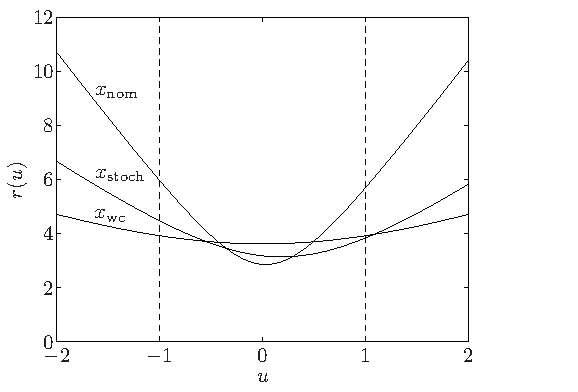
\includegraphics[width=.65\textwidth]{ch06-15.pdf}
\caption*{图6.15\quad 对三个近似解 $x$，绘出残差 $r(u)=\norm{A(u)x-b}_2$ 随不确定参数 $u$ 的变化：(1) 标称最小二乘解 $x_{\rm nom}$；(2) 随机稳健逼近问题的解 $x_{\rm stoch}$，假定 $u$ 在 $[-1,1]$ 上均匀分布；(3) 最坏情形稳健逼近问题的解 $x_{\rm wc}$，假定 $u\in[-1,1]$。标称解在 $u=0$ 时残差最小，但当 $u$ 接近 $-1$ 或 $1$ 时，残差大得多。最坏情形解在 $u=0$ 时残差较大，但当 $u$ 在 $[-1,1]$ 中变化时，残差增幅很小。}
\end{figure}
求三个近似解：
\begin{itemize}
\item \emph{标称最优解。}假定 $A(u)$ 取其标称值 $A_0$，求得最优解 $x_{\rm nom}$。
\item \emph{随机稳健逼近。}假定参数 $u$ 在 $[-1,1]$ 上均匀分布，求使 $\E\norm{A(u)x-b}_2^2$ 最小的 $x_{\rm stoch}$。
\item \emph{最坏情形稳健逼近。}求 $x_{\rm wc}$，使
\[\begin{split}\sup_{-1\le u\le1}\norm{A(u)x-b}_2
=\max\{&\norm{(A_0-A_1)x-b}_2,\\&\norm{(A_0+A_1)x-b}_2\}\end{split}\]
最小。
\end{itemize}
对这三个 $x$，图6.15分别绘出残差 $r(u)=\norm{A(u)x-b}_2$ 随不确定参数 $u$ 的变化。这些图说明，近似解可能对参数 $u$ 的变化十分敏感。标称解在 $u=0$ 时残差最小，但对参数变化颇为敏感：当 $u$ 偏离零并接近 $-1$ 或 $1$ 时，残差大得多。最坏情形解在 $u=0$ 时残差较大，但当 $u$ 在 $[-1,1]$ 内变化时，残差增幅很小。随机稳健近似解介于二者之间。
\end{origexample}
